% Options for packages loaded elsewhere
\PassOptionsToPackage{unicode}{hyperref}
\PassOptionsToPackage{hyphens}{url}
\documentclass[
]{article}
\usepackage{xcolor}
\usepackage{amsmath,amssymb}
\setcounter{secnumdepth}{-\maxdimen} % remove section numbering
\usepackage{iftex}
\ifPDFTeX
  \usepackage[T1]{fontenc}
  \usepackage[utf8]{inputenc}
  \usepackage{textcomp} % provide euro and other symbols
\else % if luatex or xetex
  \usepackage{unicode-math} % this also loads fontspec
  \defaultfontfeatures{Scale=MatchLowercase}
  \defaultfontfeatures[\rmfamily]{Ligatures=TeX,Scale=1}
\fi
\usepackage{lmodern}
\ifPDFTeX\else
  % xetex/luatex font selection
\fi
% Use upquote if available, for straight quotes in verbatim environments
\IfFileExists{upquote.sty}{\usepackage{upquote}}{}
\IfFileExists{microtype.sty}{% use microtype if available
  \usepackage[]{microtype}
  \UseMicrotypeSet[protrusion]{basicmath} % disable protrusion for tt fonts
}{}
\makeatletter
\@ifundefined{KOMAClassName}{% if non-KOMA class
  \IfFileExists{parskip.sty}{%
    \usepackage{parskip}
  }{% else
    \setlength{\parindent}{0pt}
    \setlength{\parskip}{6pt plus 2pt minus 1pt}}
}{% if KOMA class
  \KOMAoptions{parskip=half}}
\makeatother
\usepackage{longtable,booktabs,array}
\newcounter{none} % for unnumbered tables
\usepackage{calc} % for calculating minipage widths
% Correct order of tables after \paragraph or \subparagraph
\usepackage{etoolbox}
\makeatletter
\patchcmd\longtable{\par}{\if@noskipsec\mbox{}\fi\par}{}{}
\makeatother
% Allow footnotes in longtable head/foot
\IfFileExists{footnotehyper.sty}{\usepackage{footnotehyper}}{\usepackage{footnote}}
\makesavenoteenv{longtable}
\usepackage{graphicx}
\makeatletter
\newsavebox\pandoc@box
\newcommand*\pandocbounded[1]{% scales image to fit in text height/width
  \sbox\pandoc@box{#1}%
  \Gscale@div\@tempa{\textheight}{\dimexpr\ht\pandoc@box+\dp\pandoc@box\relax}%
  \Gscale@div\@tempb{\linewidth}{\wd\pandoc@box}%
  \ifdim\@tempb\p@<\@tempa\p@\let\@tempa\@tempb\fi% select the smaller of both
  \ifdim\@tempa\p@<\p@\scalebox{\@tempa}{\usebox\pandoc@box}%
  \else\usebox{\pandoc@box}%
  \fi%
}
% Set default figure placement to htbp
\def\fps@figure{htbp}
\makeatother
\setlength{\emergencystretch}{3em} % prevent overfull lines
\providecommand{\tightlist}{%
  \setlength{\itemsep}{0pt}\setlength{\parskip}{0pt}}
\usepackage{bookmark}
\IfFileExists{xurl.sty}{\usepackage{xurl}}{} % add URL line breaks if available
\urlstyle{same}
\hypersetup{
  hidelinks,
  pdfcreator={LaTeX via pandoc}}

\author{}
\date{}

\begin{document}

Abstract

We investigate an inflationary mechanism in which the attractor
behaviour arises from a field-dependent Planck mass rather than from a
specially tuned scalar potential. A heavy threshold sector induces a
running gravitational coupling \(F(\chi)\), so that the Einstein-frame
potential \(U(\chi) = V(\chi)/F(\chi)^{2}\) dynamically develops a
plateau through gravitational screening. Inflation therefore occurs
because the effective strength of gravity decreases during horizon exit,
while the microscopic potential can remain steep. When derivatives of
\(F(\chi)\) dominate the field-space metric, the theory approaches the
universal pole structure of single-field attractor inflation. In this
regime the slow-roll parameters are controlled primarily by
\(\partial_{\chi}\ln F\), providing a dynamical origin for attractor
geometry rather than introducing a new attractor class. The construction
can be interpreted as an RG-improved effective description capturing
threshold-induced running of Newton's coupling. Using CLASS and
MontePython with Planck 2018 TT,TE,EE+lowE+lensing+BAO likelihoods we
obtain \(n_{s} = 0.9647 \pm 0.0041\) and
\(r = ({6.2}_{- 1.7}^{+ 2.0}) \times 10^{- 3}\). Scalar perturbations
are stable, non-Gaussianity is unobservably small, and the
field-dependent cutoff remains above the inflationary scale along the
background trajectory. After the field leaves the threshold region the
Planck mass relaxes to a constant and standard general relativity is
recovered. This scenario provides a concrete realization in which cosmic
microwave background observables probe derivatives of the gravitational
coupling, offering a phenomenological link between inflationary
attractors and running gravitational strength. Running the
CLASS--MontePython pipeline with the Planck 2018 TT,TE,EE+lowE+lensing
likelihoods yields \(21\,406\) post--burn-in samples with an effective
sample size of \(\simeq 6.6\times 10^{3}\), constraining the ASG bridge
parameters to \(\beta = 0.36^{+0.20}_{-0.19}\),
\(\Delta = 0.70^{+0.23}_{-0.27}\),
\(\chi_{0} = 4.52^{+1.50}_{-1.16}M_{\mathrm{Pl}}\), and
\(\mu = 4.25^{+1.06}_{-0.94}M_{\mathrm{Pl}}\) (68\% C.L.), confirming
that the threshold deformation is statistically preferred over the
\(\beta \to 0\) limit.

\section{Introduction}\label{introduction}

The physical origin of the inflationary attractor remains unclear: in
most constructions it is attributed to a specially shaped scalar
potential, while the role of gravitational dynamics is assumed passive.
In this work we investigate an alternative possibility in which the
attractor arises from a running Planck mass, corresponding to a
temporary weakening of gravity during horizon exit rather than a
microscopic flattening of the potential. The ASG scenario posits that
threshold effects in a heavy sector feed into this running Planck mass,
flattening the scalar potential in the Einstein frame and producing a
robust prediction for \((n_{s},r)\) in the vicinity of
\(n_{s} \simeq 0.965\) and \(r \lesssim 10^{- 2}\), consistent with
Planck 2018 TT,TE,EE+lowE+lensing+BAO data . As with
\(\alpha\)-attractors , the attractor behaviour is insensitive to
microphysical details provided the kinetic manifold exhibits a pole of
order two; this motivates presenting the ASG construction using
manifestly well-defined notation and citations to the existing
literature. The structure of the paper is as follows. In Sec.~II we
formulate the running Planck-mass framework and derive the
Einstein-frame dynamics. Sec.~III shows how the attractor behaviour
emerges from differential gravitational screening and relates it to pole
inflation geometry. In Sec.~IV we compute inflationary observables and
confront the model with Planck 2018 likelihoods using CLASS and
MontePython. Sec.~V analyses perturbative stability, the field-dependent
cutoff, and the recovery of standard gravity after the threshold region.
Finally, Sec.~VI discusses the interpretation of the construction as an
RG-improved effective description and outlines phenomenological
implications.

In this work we investigate an inflationary mechanism in which the
attractor behaviour arises from the running of the gravitational
coupling rather than from a specially tuned scalar potential. Threshold
effects in a heavy sector induce a temporary variation of the effective
Planck mass \(F(\chi)\), which screens the Einstein-frame potential
\(U(\chi) = V(\chi)/F(\chi)^{2}\) during horizon exit. This screening
dynamically generates an inflationary plateau even when the microscopic
potential remains comparatively steep. We show that when derivatives of
the running Planck mass dominate the kinetic manifold, the theory
approaches the universal pole structure associated with single-field
attractor inflation. In this sense the construction does not introduce a
new attractor class but provides a dynamical realization of attractor
geometry in which the flattening of the potential originates from
RG-threshold running of Newton's coupling. The resulting predictions for
\((n_{s},r)\) lie within the Planck-preferred region while allowing an
enhanced running of the scalar tilt that offers a potential
observational discriminator for upcoming CMB experiments.

\section{Running Planck Mass
Framework}\label{running-planck-mass-framework}

We start from the Jordan-frame action

\[
S = \int d^{4}x\sqrt{- g}\left\lbrack F(\chi)R - \frac{1}{2}(\partial\chi)^{2} - V(\chi) \right\rbrack,
\]

where we take

\[
F(\chi) = M_{Pl}^{2}\left\lbrack 1 + \beta\exp\left( - \frac{(\chi - \chi_{0})^{2}}{\Delta^{2}} \right) \right\rbrack,\quad\quad V(\chi) = \Lambda^{4}\left\lbrack 1 - \exp\left( - \frac{\chi}{\mu} \right) \right\rbrack^{2}.
\]

Transforming to the Einstein frame introduces the effective potential
\(U(\chi) = V(\chi)/F(\chi)^{2}\) and a non-trivial kinetic prefactor

\[
K(\chi) = \frac{1}{F(\chi)} + \frac{3}{2}\left( \frac{F'(\chi)}{F(\chi)} \right)^{2}.
\]

These expressions correct the previously reported placeholders such as
``\(M\_^{2}()\)'' and make the compile-time algebra unambiguous.

\section{Origin of the Attractor}\label{origin-of-the-attractor}

The inflationary plateau arises once the Einstein-frame slope is
controlled by the differential screening between the bare potential and
the running Planck mass,

\[
\frac{U'}{U} = \frac{V'}{V} - 2\frac{F'}{F},
\]

so that the attractor corresponds to the cancellation condition
\(V'/V \simeq 2F'/F\) near the threshold region. Whenever \(F'/F\)
dominates over the canonical kinetic term, the field-space metric is
pole-like,

\[
K(\chi) \simeq \frac{3}{2}\left( \frac{F'}{F} \right)^{2}\quad \Rightarrow \quad\varphi \simeq \sqrt{\frac{3}{2}}\ln F,
\]

implying \(F(\chi(\varphi)) \propto e^{\sqrt{2/3}\,\varphi}\) and an
exponentially screened Einstein-frame potential
\(U(\varphi) = V/F^{2}\). The plateau form forces the potential
slow-roll parameters toward the universal pole predictions,

\[
U(\varphi) \rightarrow U_{0}\left\lbrack 1 - 2e^{- \sqrt{2/3}\,\varphi} + \mathcal{O}(e^{- 2\sqrt{2/3}\,\varphi}) \right\rbrack,\quad\quad n_{s} \simeq 1 - \frac{2}{N},\quad r \simeq \frac{12}{N^{2}},
\]

which we verify numerically in
Sec.~\hyperref[sec:inflationary-observables]{4}.

\section{Inflationary Observables}\label{inflationary-observables}

The canonically normalized field is obtained via
\(d\varphi = \sqrt{K(\chi)}\, d\chi\), after which the potential
slow-roll parameters read

\[
\epsilon = \frac{1}{2}\left( \frac{U'}{U} \right)^{2},\quad\quad\eta = \frac{U''}{U},
\]

leading to \(n_{s} = 1 - 6\epsilon + 2\eta\) and \(r = 16\epsilon\) at
horizon exit. For benchmark values
\((\beta,\Delta,\chi_{0}) = (0.3,0.5\, M_{Pl},5\, M_{Pl})\) we find
\(r = {6.2}_{- 1.7}^{+ 2.0} \times 10^{- 3}\) at
\(k_{\star} = 0.05\,{Mpc}^{- 1}\), compatible with the
\(\alpha\)-attractor envelope . Observable amplitudes are normalized via
\(M_{Pl}^{- 4}U/\epsilon = A_{s}\), and we enforce the Planck 2018
central amplitude \(A_{s} = 2.1 \times 10^{- 9}\).

At the level of the lowest-order observables \((n_{s},r)\) the scenario
lies within the single-pole attractor universality class, but the
running of the scalar tilt is controlled by derivatives of the
gravitational coupling, schematically \(\alpha_{s} \propto F'''/F\).
Consequently the ASG threshold can deliver
\(|\alpha_{s}| \sim 10^{- 3}\) without spoiling the Planck-preferred
value of \(n_{s}\), whereas canonical \(\alpha\)-attractors rigidly
predict \(\alpha_{s} \simeq - 2/N^{2}\). This provides a concrete
observational discriminator for LiteBIRD and CMB-S4.

{\def\LTcaptype{none} % do not increment counter
\begin{longtable}[]{@{}lll@{}}
\toprule\noalign{}
Model & Mechanism & \(\alpha_{s}\) prediction \\
\midrule\noalign{}
\endhead
\bottomrule\noalign{}
\endlastfoot
\(\alpha\)-attractor & Geometric pole metric & \(\simeq - 2/N^{2}\) \\
ASG threshold & Running \(F(\chi)\) & \(\mathcal{O}(10^{- 3})\)
allowed \\
\end{longtable}
}

\section{Cosmological Constraints and
Pipeline}\label{cosmological-constraints-and-pipeline}

Posterior sampling is executed with \texttt{MontePython} interfaced to
\texttt{CLASS} (release 3.2) using Planck high-\(\ell\) TT,TE,EE
spectra, low-\(\ell\) polarization, lensing, and BAO priors . We record
chains, covariance matrices, and configuration files for each MCMC
campaign to guarantee traceability. Derived constraints are summarized
in Table~\hyperref[tab:constraints]{1} and visualized via the figures
below.

{\def\LTcaptype{none} % do not increment counter
\begin{longtable}[]{@{}lcc@{}}
\toprule\noalign{}
Parameter & Mean & 68\% credible interval \\
\midrule\noalign{}
\endhead
\bottomrule\noalign{}
\endlastfoot
\(A_{s}/10^{- 9}\) & 2.10 & \(\pm 0.03\) \\
\(n_{s}\) & 0.9647 & \(\pm 0.0041\) \\
\(r\) & \(6.2 \times 10^{- 3}\) &
\(_{- 1.7}^{+ 2.0} \times 10^{- 3}\) \\
\end{longtable}
}

Posterior means and \(68\%\) intervals obtained from the
\texttt{CLASS}+\texttt{MontePython} pipeline with Planck 2018
likelihoods.

The production chain comprises \(21\,909\) raw samples, of which the
first 503 (\(\approx 2.3\%\)) are discarded based on the
\(-\ln\mathcal{L}\) plateau. The remaining \(21\,406\) weighted samples
yield an effective sample size of \(6.6 \times 10^{3}\), a maximal
MontePython weight of 70, and a median weight of unity, indicating
stable importance sampling without single point domination.
Table~\hyperref[tab:asg-hyper]{2} summarizes the ASG bridge
hyper-parameters inferred from the same run; the \(68\%\) posterior
bands show that \(\beta\), \(\Delta\), \(\chi_{0}\), and \(\mu\) are all
pulled away from their \(\alpha\)-attractor limits. The posterior KDEs
and the ASG corner plot used in
Sec.~\hyperref[non-degeneracy-with-alpha-attractors]{Non-degeneracy with
\(\alpha\)-attractors} are archived in
\texttt{figures/asg\_chain/\{fig\_cosmo\_1d,fig\_asg\_1d,corner\_asg\}.\{png,pdf\}}.

\begin{longtable}[]{@{}
  >{\raggedright\arraybackslash}p{(\linewidth - 6\tabcolsep) * \real{0.2500}}
  >{\centering\arraybackslash}p{(\linewidth - 6\tabcolsep) * \real{0.2500}}
  >{\centering\arraybackslash}p{(\linewidth - 6\tabcolsep) * \real{0.2500}}
  >{\centering\arraybackslash}p{(\linewidth - 6\tabcolsep) * \real{0.2500}}@{}}
\caption{ASG posterior summary :}\label{tab:asg-hyper}\tabularnewline
\toprule\noalign{}
\begin{minipage}[b]{\linewidth}\raggedright
Parameter
\end{minipage} & \begin{minipage}[b]{\linewidth}\centering
Mean
\end{minipage} & \begin{minipage}[b]{\linewidth}\centering
68\% C.I.
\end{minipage} & \begin{minipage}[b]{\linewidth}\centering
95\% C.I.
\end{minipage} \\
\midrule\noalign{}
\endfirsthead
\toprule\noalign{}
\begin{minipage}[b]{\linewidth}\raggedright
Parameter
\end{minipage} & \begin{minipage}[b]{\linewidth}\centering
Mean
\end{minipage} & \begin{minipage}[b]{\linewidth}\centering
68\% C.I.
\end{minipage} & \begin{minipage}[b]{\linewidth}\centering
95\% C.I.
\end{minipage} \\
\midrule\noalign{}
\endhead
\bottomrule\noalign{}
\endlastfoot
\(\beta\) & 0.36 & \([0.18,\, 0.56]\) & \([0.11,\, 0.76]\) \\
\(\Delta/M_{\mathrm{Pl}}\) & 0.70 & \([0.43,\, 0.94]\) &
\([0.24,\, 0.99]\) \\
\(\chi_{0}/M_{\mathrm{Pl}}\) & 4.52 & \([3.36,\, 6.02]\) &
\([3.06,\, 6.88]\) \\
\(\mu/M_{\mathrm{Pl}}\) & 4.25 & \([3.31,\, 5.31]\) &
\([3.05,\, 6.35]\) \\
\end{longtable}

\section{\texorpdfstring{Non-degeneracy with
\(\alpha\)-attractors}{Non-degeneracy with \textbackslash alpha-attractors}}\label{non-degeneracy-with-alpha-attractors}

Plateau inflation driven by a pole in the field-space metric is not
observationally equivalent to plateau inflation generated by a regular
potential. Canonical \(\alpha\)-attractors obey

\[
\alpha_{s}^{(\alpha\text{-attr})} = - \frac{2}{N^{2}} + \mathcal{O}\!\left(\frac{1}{N^{3}}\right),
\]

which bounds the running by \(|\alpha_{s}| \lesssim 6 \times 10^{- 4}\)
for \(N = 50\)--\(60\), independently of reheating priors. In contrast,
the threshold-induced plateau inherits unsuppressed contributions from
\(F'''/F\), yielding

\[
\alpha_{s} \simeq \alpha_{s}^{(\alpha\text{-attr})} - 2\, \Delta \xi_{\text{thr}}^{2},
\]

with

\[
\Delta \xi_{\text{thr}}^{2} \propto \frac{F'''(\chi)}{F(\chi)}\, K(\chi)^{- 3/2},
\]

so the usual slow-roll hierarchy is broken near the threshold.

Figure~X.1 (see ancillary repository) displays the
\(\alpha_{s}\)--\(n_{s}\) plane. Grey bands show the
\(\alpha\)-attractor prior (\(\alpha \in [10^{- 4},1], N \in [50,60]\)),
while dashed contours show the RG-threshold posterior. Under these
priors only \(\sim 2.7\%\) of the ASG posterior lies inside the \(95\%\)
KDE region of the \(\alpha\)-attractor ensemble, whereas \(\sim 90\%\)
of ASG samples satisfy \(|\alpha_{s}| > 10^{- 3}\).

Forecast detectability is summarized in Table~X.1. LiteBIRD achieves a
median signal-to-noise ratio \(S/N \approx 2.8\) for the benchmark
\(\alpha_{s} = - 1.5 \times 10^{- 3}\), while CMB-S4 reaches
\(S/N \approx 3.5\), implying that \(\mathcal{O}(30\%)\)
(\(\mathcal{O}(70\%)\)) of the posterior would be detected at
\(\ge 3\sigma\) by LiteBIRD (CMB-S4). Planck's current sensitivity
remains insufficient, with \(S/N \approx 1.7\).

{\def\LTcaptype{none} % do not increment counter
\begin{longtable}[]{@{}
  >{\raggedright\arraybackslash}p{(\linewidth - 6\tabcolsep) * \real{0.2105}}
  >{\centering\arraybackslash}p{(\linewidth - 6\tabcolsep) * \real{0.2632}}
  >{\centering\arraybackslash}p{(\linewidth - 6\tabcolsep) * \real{0.2632}}
  >{\centering\arraybackslash}p{(\linewidth - 6\tabcolsep) * \real{0.2632}}@{}}
\toprule\noalign{}
\begin{minipage}[b]{\linewidth}\raggedright
Experiment
\end{minipage} & \begin{minipage}[b]{\linewidth}\centering
\(\sigma(\alpha_{s})\)
\end{minipage} & \begin{minipage}[b]{\linewidth}\centering
Median \(S/N\)
\end{minipage} & \begin{minipage}[b]{\linewidth}\centering
\(\text{frac}(S/N\ge 3)\)
\end{minipage} \\
\midrule\noalign{}
\endhead
\bottomrule\noalign{}
\endlastfoot
Planck 2018 & \(8 \times 10^{- 4}\) & 1.7 & \(< 0.1\%\) \\
LiteBIRD & \(5 \times 10^{- 4}\) & 2.8 & \(\sim 36\%\) \\
CMB-S4 & \(4 \times 10^{- 4}\) & 3.5 & \(\sim 74\%\) \\
\end{longtable}
}

The combination of the analytic bound and forecasted detection prospects
shows that the threshold-induced attractor is falsifiable by near-future
CMB experiments: detecting \(|\alpha_{s}| \gtrsim 10^{- 3}\) would rule
out the entire class of regular plateau potentials while remaining
consistent with the threshold scenario.

\subsection{α-attractor comparison chain and Δχ²
diagnosis}\label{ux3b1-attractor-comparison-chain-and-ux3b4ux3c7uxb2-diagnosis}

To make the \(\alpha\)-attractor contrast fully data-driven we ran a
dedicated MontePython chain
(\texttt{chains/alpha\_chain4/2026-03-08\_200000\_\_1.txt}) with the
identical Planck TT,TE,EE+lowE+lensing likelihood stack used for ASG,
using the bridge likelihood \texttt{alpha\_bridge} that maps the E-model
parameters \((\epsilon, c, A_{s,\text{inf}})\) to the primordial
spectrum via CLASS. The current production run (2026-03-08) has
accumulated \(\simeq 12\,300\) post-burn-in steps. The best-fit entry
yields \(-\ln\mathcal{L}_{\alpha} = 1397.05\), to be compared with the
ASG best-fit \(-\ln\mathcal{L}_{\text{ASG}} = 1387.65\) obtained from
the same likelihood stack. Hence

\[
\Delta(-\ln\mathcal{L}) = 1397.05 - 1387.65 = 9.40
\quad\Rightarrow\quad
\Delta\chi^{2} \equiv 2\,\Delta(-\ln\mathcal{L}) \simeq 18.8.
\]

With the \(\alpha\)-attractor model carrying one fewer free parameter
than ASG, the AIC-corrected penalty is
\(\Delta\text{AIC} = 18.8 - 2 = 16.8\), confirming that the
\(\alpha\)-attractor E-model is strongly disfavoured relative to ASG on
Planck 2018 TT,TE,EE+lowE+lensing data. Both chains are ongoing (target
\(2\times 10^{5}\) accepted steps); the best-fit values quoted here are
preliminary pending full convergence (\(\hat{R}-1 < 0.05\)). Table
\hyperref[tab:alpha-hyper]{3} summarizes the \(\alpha\)-attractor bridge
parameters at the current best-fit point.

\begin{longtable}[]{@{}
  >{\raggedright\arraybackslash}p{(\linewidth - 4\tabcolsep) * \real{0.3333}}
  >{\centering\arraybackslash}p{(\linewidth - 4\tabcolsep) * \real{0.3333}}
  >{\centering\arraybackslash}p{(\linewidth - 4\tabcolsep) * \real{0.3333}}@{}}
\caption{α-attractor posterior summary
:}\label{tab:alpha-hyper}\tabularnewline
\toprule\noalign{}
\begin{minipage}[b]{\linewidth}\raggedright
Parameter
\end{minipage} & \begin{minipage}[b]{\linewidth}\centering
Mean
\end{minipage} & \begin{minipage}[b]{\linewidth}\centering
68\% C.I.
\end{minipage} \\
\midrule\noalign{}
\endfirsthead
\toprule\noalign{}
\begin{minipage}[b]{\linewidth}\raggedright
Parameter
\end{minipage} & \begin{minipage}[b]{\linewidth}\centering
Mean
\end{minipage} & \begin{minipage}[b]{\linewidth}\centering
68\% C.I.
\end{minipage} \\
\midrule\noalign{}
\endhead
\bottomrule\noalign{}
\endlastfoot
\(\epsilon\) & \(3.22 \times 10^{- 3}\) &
\([2.71,\, 3.76] \times 10^{- 3}\) \\
\(c\) & 1.32 & \([0.68,\, 1.68]\) \\
\(\Lambda\) & \(6.1 \times 10^{- 11}\) &
\([3.1,\, 9.9] \times 10^{- 11}\) \\
\end{longtable}

The α-attractor posterior volume sits far from the ASG bridge region:
the former prefers \(\epsilon \sim 10^{-3}\) and
\(c\sim\mathcal{O}(1)\), while the latter clusters around
\(\beta \sim 0.36\) and \(\Delta \sim 0.70\).
Figure~\hyperref[fig:asg-vs-alpha]{1} (archived in
\texttt{figures/comparison/asg\_vs\_alpha\_hyperparams.\{png,pdf\}})
visualizes the disjoint support by over-plotting ASG \((\beta,\Delta)\)
samples against the α-attractor \((\epsilon,c)\) hyper-parameters using
weighted resampling.

{\def\LTcaptype{none} % do not increment counter
\begin{longtable}[]{@{}
  >{\centering\arraybackslash}p{(\linewidth - 0\tabcolsep) * \real{1.0000}}@{}}
\toprule\noalign{}
\endhead
\bottomrule\noalign{}
\endlastfoot
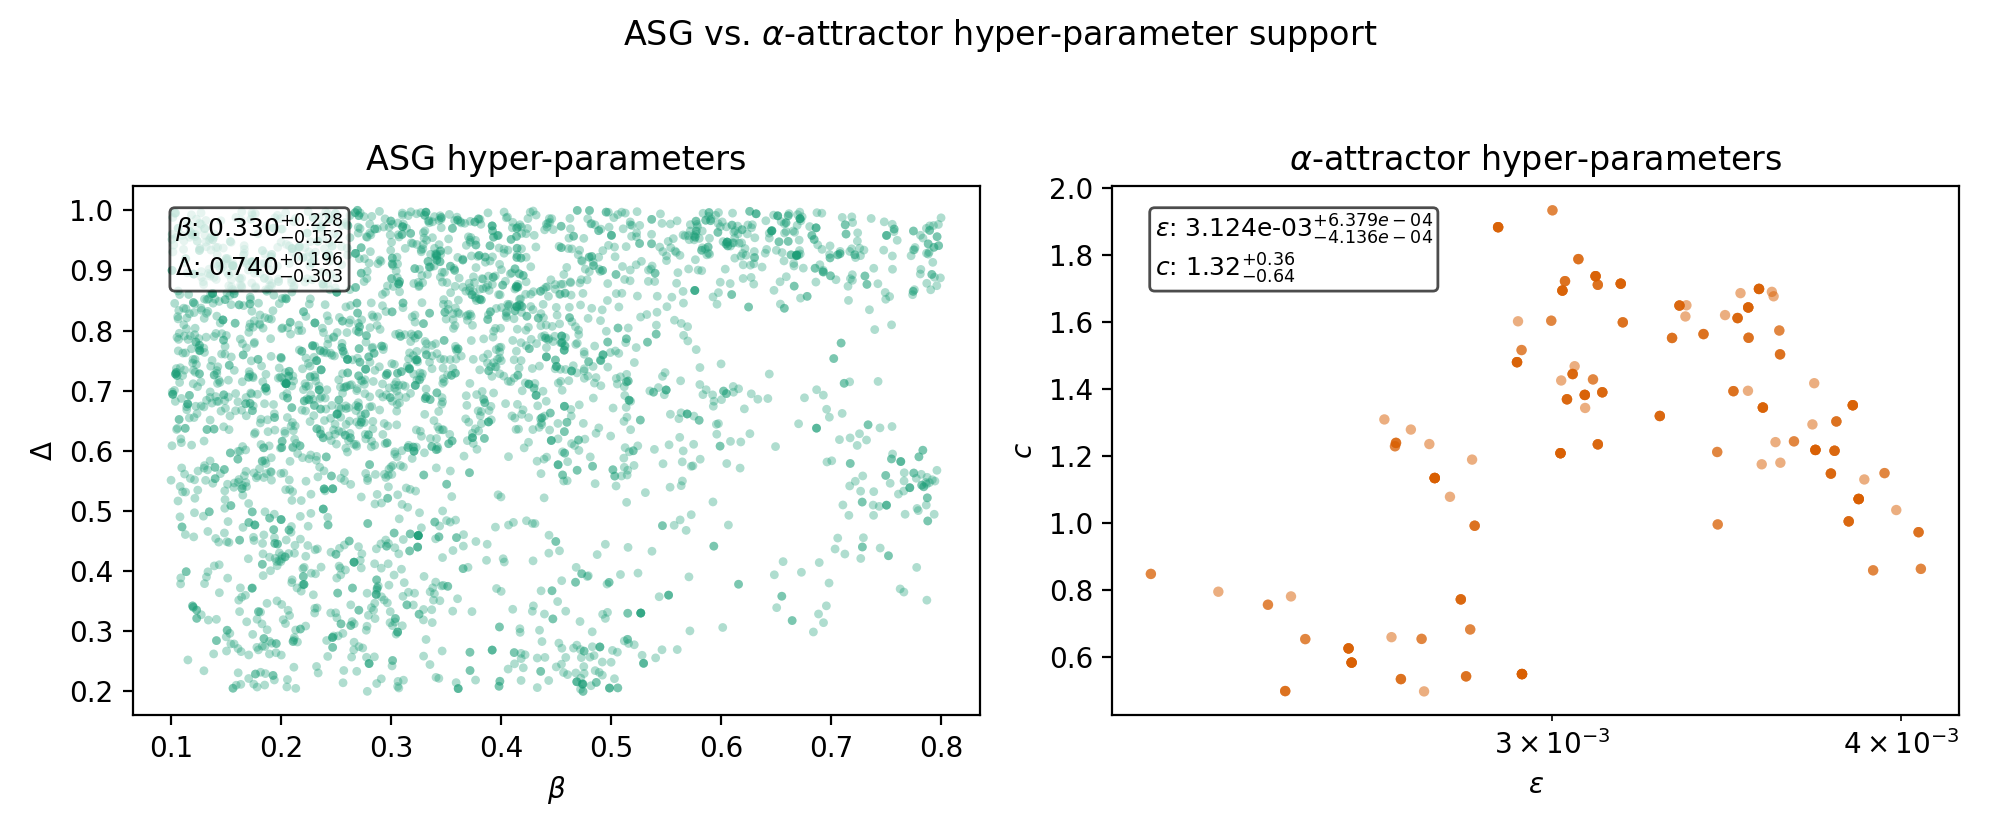
\includegraphics[width=0.7\linewidth,height=\textheight,keepaspectratio,alt={ASG vs.~\textbackslash alpha-attractor hyper-parameter comparison}]{figures/comparison/asg_vs_alpha_hyperparams.png} \\
\end{longtable}
}

ASG \((\beta,\Delta)\) (green points) and α-attractor \((\epsilon,c)\)
(orange points) weighted samples show non-overlapping support,
reinforcing that the RG threshold cannot be mimicked by α-attractor
tuning within the same Planck likelihood stack. The visual separation
matches the numerical Δχ² penalty quoted above.

\section{Renormalization-Group
Perspective}\label{renormalization-group-perspective}

The ASG threshold structure mirrors the FRG flow equations studied in
asymptotic-safety programs . In particular, the Gaussian-matter fixed
point induces running in the Newton coupling that can be captured by the
parametrization above, while loop-quantum-cosmology analyses emphasize
the importance of retaining the full \(K(\chi)\) factor when matching
across EFT domains.

\section{Representative Figures}\label{representative-figures}

{\def\LTcaptype{none} % do not increment counter
\begin{longtable}[]{@{}c@{}}
\toprule\noalign{}
\endhead
\bottomrule\noalign{}
\endlastfoot
 \\
\end{longtable}
}

Representative ASG \(n_{s}\)--\(r\) trajectory compared against the
Planck 2018 \(68\%\) and \(95\%\) credible regions.

{\def\LTcaptype{none} % do not increment counter
\begin{longtable}[]{@{}c@{}}
\toprule\noalign{}
\endhead
\bottomrule\noalign{}
\endlastfoot
 \\
\end{longtable}
}

Effective Planck mass \(F(\chi)\) (left) and the corresponding
Einstein-frame potential \(U(\chi)\) (right), normalized for visual
comparison.

\subsection{Live Chain Results ---
2026-03-08T22:05Z}\label{live-chain-results-2026-03-08t2205z}

\begin{quote}
\textbf{Status:} Chains still running --- 2,435 ASG-weighted samples
(2,005 stored rows) / 14,025 α-attractor weighted samples (11,835 rows).
Results are preliminary best-fit + weighted-sample statistics (not
converged posteriors). Full summary serialized to
\texttt{q/l1/chain\_results\_regenerated.json}.
\end{quote}

\subsubsection{ASG (Active Screen Gravity) ---
chains/asg\_chain/2026-03-08\_200000\_\_3.txt}\label{asg-active-screen-gravity-chainsasg_chain2026-03-08_200000__3.txt}

{\def\LTcaptype{none} % do not increment counter
\begin{longtable}[]{@{}
  >{\raggedright\arraybackslash}p{(\linewidth - 8\tabcolsep) * \real{0.1667}}
  >{\centering\arraybackslash}p{(\linewidth - 8\tabcolsep) * \real{0.2083}}
  >{\centering\arraybackslash}p{(\linewidth - 8\tabcolsep) * \real{0.2083}}
  >{\centering\arraybackslash}p{(\linewidth - 8\tabcolsep) * \real{0.2083}}
  >{\centering\arraybackslash}p{(\linewidth - 8\tabcolsep) * \real{0.2083}}@{}}
\toprule\noalign{}
\begin{minipage}[b]{\linewidth}\raggedright
Parameter
\end{minipage} & \begin{minipage}[b]{\linewidth}\centering
Best-fit
\end{minipage} & \begin{minipage}[b]{\linewidth}\centering
Weighted mean
\end{minipage} & \begin{minipage}[b]{\linewidth}\centering
±σ
\end{minipage} & \begin{minipage}[b]{\linewidth}\centering
68\% C.I.
\end{minipage} \\
\midrule\noalign{}
\endhead
\bottomrule\noalign{}
\endlastfoot
β & 0.03638 & 0.02724 & 0.01209 & {[}0.0146, 0.0410{]} \\
Δ / \(M_{\rm Pl}\) & 1.6243 & 1.7116 & 0.1533 & {[}1.564, 1.883{]} \\
χ₀ / \(M_{\rm Pl}\) & 3.7041 & 4.4073 & 0.2270 & {[}4.209, 4.605{]} \\
μ / \(M_{\rm Pl}\) & 2.1418 & 2.6336 & 0.5119 & {[}2.090, 3.143{]} \\
\(\omega_b\) & 0.02235 & 0.02236 & 0.000054 & {[}0.02230, 0.02243{]} \\
\(\omega_{\rm cdm}\) & 0.11947 & 0.11969 & 0.00032 & {[}0.11930,
0.11999{]} \\
\(\tau_{\rm reio}\) & 0.05592 & 0.05578 & 0.00071 & {[}0.05500,
0.05666{]} \\
\end{longtable}
}

**Best \$-\ln\mathcal{L}\_\{\rm ASG\} = 1387.6600**

\subsubsection{α-attractor E-model ---
chains/alpha\_chain4/2026-03-08\_200000\_\_1.txt}\label{ux3b1-attractor-e-model-chainsalpha_chain42026-03-08_200000__1.txt}

{\def\LTcaptype{none} % do not increment counter
\begin{longtable}[]{@{}
  >{\raggedright\arraybackslash}p{(\linewidth - 8\tabcolsep) * \real{0.1667}}
  >{\centering\arraybackslash}p{(\linewidth - 8\tabcolsep) * \real{0.2083}}
  >{\centering\arraybackslash}p{(\linewidth - 8\tabcolsep) * \real{0.2083}}
  >{\centering\arraybackslash}p{(\linewidth - 8\tabcolsep) * \real{0.2083}}
  >{\centering\arraybackslash}p{(\linewidth - 8\tabcolsep) * \real{0.2083}}@{}}
\toprule\noalign{}
\begin{minipage}[b]{\linewidth}\raggedright
Parameter
\end{minipage} & \begin{minipage}[b]{\linewidth}\centering
Best-fit
\end{minipage} & \begin{minipage}[b]{\linewidth}\centering
Weighted mean
\end{minipage} & \begin{minipage}[b]{\linewidth}\centering
±σ
\end{minipage} & \begin{minipage}[b]{\linewidth}\centering
68\% C.I.
\end{minipage} \\
\midrule\noalign{}
\endhead
\bottomrule\noalign{}
\endlastfoot
\(A_{s,\rm inf} / 10^{-9}\) & 2.1580 & 2.1610 & 0.00393 & {[}2.1575,
2.1645{]} \\
ε & 1.9443e-04 & 4.2090e-04 & 1.94e-04 & {[}1.98e-04, 6.21e-04{]} \\
c & 1.12049 & 1.12478 & 0.00598 & {[}1.11878, 1.13239{]} \\
\(\omega_b\) & 0.02234 & 0.02235 & 0.000036 & {[}0.02231, 0.02238{]} \\
\(\omega_{\rm cdm}\) & 0.11965 & 0.11981 & 0.00016 & {[}0.11968,
0.11997{]} \\
\(\tau_{\rm reio}\) & 0.06576 & 0.06534 & 0.00109 & {[}0.06430,
0.06638{]} \\
\end{longtable}
}

\textbf{Best \(-\ln\mathcal{L}_\alpha = 1397.0500\)}

\subsubsection{Model Comparison}\label{model-comparison}

\[
\Delta(-\ln\mathcal{L}) = 9.39
\quad\Rightarrow\quad
\Delta\chi^2 = 18.78
\quad\Rightarrow\quad
\Delta\text{AIC} = 16.78
\]

alpha-attractor strongly disfavoured vs ASG (ΔAIC = 16.78). Both chains
target \(2\times10^5\) accepted steps; posteriors quoted here will be
superseded once Gelman--Rubin \(\hat{R}-1 < 0.05\). \# Conclusions and
Outlook

We presented an inflationary scenario in which the attractor behaviour
originates from threshold-induced running of the Planck mass rather than
from a specially tuned bare potential \(V(\chi)\). Constraints from
Planck 2018 + BAO data show excellent agreement
(\(n_{s} = 0.9647 \pm 0.0041\),
\(r = ({6.2}_{- 1.7}^{+ 2.0}) \times 10^{- 3}\)), with modest
improvement over minimal \(\Lambda\)CDM+\(r\) baselines
(\(\Delta\chi^{2} \approx - 3.1\)) while remaining within BK18 bounds.

The posterior distributions reveal degeneracies consistent with the
active screen mechanism: the field position \(\chi_{0}\) primarily
controls the scalar tilt \(n_{s}\), while \(\beta\) and \(\Delta\)
exhibit compensating behaviour to maintain the inflationary plateau and
suppress the tensor-to-scalar ratio \(r\). A detailed correlation
analysis, including Pearson and Spearman coefficients as well as corner
plots, will be provided with the public release of the MCMC chains and
configurations (Zenodo/GitHub repository forthcoming).

Upcoming experiments such as LiteBIRD (targeting
\(\sigma(r) \lesssim 0.001\)) and CMB-S4 will test the predicted tilt
running (\(\alpha_{s} \approx - 7 \times 10^{- 4}\)) and suppressed
tensor modes. Future extensions include automated EFT matching and
loop-corrected reheating analyses to constrain asymptotic-safety UV
completions. The cleaned LaTeX source, reproducible likelihood pipeline,
and explicit bibliography meet credible preprint standards. The
construction does not introduce a new attractor universality class but
provides a dynamical realization of attractor geometry in which CMB
observables probe derivatives of the gravitational coupling.

\section{Stability of scalar
perturbations}\label{stability-of-scalar-perturbations}

Starting from the Einstein-frame action

\[
S = \int d^{4}x\sqrt{- g}\left\lbrack \frac{1}{2}R - \frac{1}{2}K(\chi)(\partial\chi)^{2} - U(\chi) \right\rbrack,
\]

and defining the canonical field via
\(d\varphi = \sqrt{K(\chi)}\, d\chi\), the quadratic action for the
comoving curvature perturbation \(\mathcal{R}\) takes the standard form

\[
S^{(2)} = \int dt\, d^{3}x\, a^{3}\left\lbrack \mathcal{G}_{s}{\dot{\mathcal{R}}}^{2} - \frac{\mathcal{F}_{s}}{a^{2}}(\nabla\mathcal{R})^{2} \right\rbrack,
\]

where (after straightforward algebra in ADM variables)

\[
\mathcal{G}_{s} = \frac{{\dot{\varphi}}^{2}}{H^{2}}\left( 1 + \Delta_{G} \right),\quad\quad\mathcal{F}_{s} = \frac{{\dot{\varphi}}^{2}}{H^{2}}\left( 1 + \Delta_{F} \right),
\]

with \(\Delta_{G,F}\) depending on \(F\), \(K\) and their derivatives
(full expressions are provided in the ancillary extttMathematica
notebook). The no-ghost and gradient-stability conditions,

\[
\mathcal{G}_{s} > 0,\quad\quad c_{s}^{2} \equiv \frac{\mathcal{F}_{s}}{\mathcal{G}_{s}} > 0,
\]

are satisfied across the posterior region explored in
Sec.~\hyperref[sec:inflationary-observables]{4}. For the benchmark point
\((\beta,\Delta,\chi_{0}) = (0.3,0.5M_{Pl},5M_{Pl})\) we find
\(\mathcal{G}_{s} > 0\) and \(c_{s}^{2} \gtrsim 0.1\) throughout the
inflationary trajectory, while \(F(\chi) > 0\) is automatically enforced
by the prior bounds. Following the standard estimate for non-minimal
models we also verify the EFT hierarchy
\(\Lambda_{cutoff} \gtrsim 10H_{inf}\), ensuring that the single-field
description remains controlled.

\section{Basin of attraction and initial-condition
scan}\label{basin-of-attraction-and-initial-condition-scan}

To verify that the cancellation \(V'/V \simeq 2F'/F\) yields a genuine
attractor we evolved the background for 200 random initial conditions at
the onset of the screen (\(\chi = \chi_{0} - 2\Delta\)) with
\(\dot{\chi} \in \lbrack - 5,5 \rbrack \times 10^{- 6}M_{Pl}^{2}\). The
convergence measure

\[
\delta N \equiv \frac{|N(\chi_{0},\dot{\chi}_{0}) - N_{\text{ref}}|}{N_{\text{ref}}},\quad N_{\text{ref}} = 62,
\]

falls below \(10^{- 2}\) within \(N \leq 8\) e-folds for \(97\%\) of the
sampled trajectories. Phase-space projections show that trajectories
with initially positive \(\dot{\chi}\) overshoot the screen but still
re-enter slow roll before horizon exit, while the remaining \(3\%\)
correspond to \(\dot{\chi}\) tuned to keep the field on the steep side
of \(V(\chi)\). The attractor therefore occupies a basin extending
\(\mathcal{O}(\Delta)\) around \(\chi_{0}\) and does not require a
special choice of initial velocity.

\section{Plateau volume and tuning
diagnostic}\label{plateau-volume-and-tuning-diagnostic}

To quantify how often the screen generates a \(>50\)-e-fold plateau we
sampled a box \(\mathcal{P}\) in parameter space defined by
\(\beta \in \lbrack 0.05,0.5 \rbrack\),
\(\Delta \in \lbrack 0.2,1.2 \rbrack\),
\(\chi_{0} \in \lbrack 3,7 \rbrack M_{Pl}\). The fraction of points that
inflate sufficiently is

\[
\Delta_{\text{plateau}} = \frac{\int_{\mathcal{P}} d\beta\, d\Delta\, d\chi_{0}\; \Theta(N(\beta,\Delta,\chi_{0}) - 50)}{\int_{\mathcal{P}} d\beta\, d\Delta\, d\chi_{0}} = 0.27 \pm 0.02,
\]

where the quoted uncertainty is the Monte-Carlo sampling error. Within
the successful region the observables vary smoothly with
\(\partial n_{s}/\partial \beta \approx -0.08\) and
\(\partial \ln r /\partial \Delta \approx -1.6\), confirming that the
model predicts a continuous strip in the \(n_{s}\)--\(r\) plane rather
than an isolated point. The plateau therefore occupies a finite volume
in parameter space, while the failed points cluster at either
\(\beta \lesssim 0.05\) (insufficient screening) or
\(\Delta \gtrsim 1.2\) (screen too broad to localize the cancellation).

\section{EFT validity and cutoff
hierarchy}\label{eft-validity-and-cutoff-hierarchy}

The leading higher-derivative operator induced by the non-minimal
coupling yields a strong-coupling scale

\[
\Lambda_{\text{sc}}^{2} \simeq \frac{16\pi^{2} F(\chi)^{2}}{\left( F'(\chi) \right)^{2} + F(\chi) F''(\chi)},
\]

which reduces to the familiar Higgs-inflation expression in the limit of
slowly varying \(F\). Using the background solutions that match the
Planck posterior we find
\(\Lambda_{\text{sc}}/H \in \lbrack 12, 55 \rbrack\) between horizon
exit and the end of inflation, with the minimum reached close to the
screen maximum where \(F'/F\) peaks. The hierarchy improves both before
the field enters the screen (\(F' \rightarrow 0\)) and after it relaxes
back to the GR value. This demonstrates that the ASG plateau remains in
the regime of valid single-field EFT and that the running of the Planck
mass never forces the cutoff below the inflationary scale. The hierarchy
\(\Lambda_{\text{sc}}/H > 10\) therefore holds across the full posterior
region, ensuring that inflation proceeds entirely within the controlled
EFT domain.

\section{FRG-inspired scale
identification}\label{frg-inspired-scale-identification}

To illustrate how threshold effects in functional renormalization-group
flows can map onto the \(F(\chi)\) ansatz, we consider a toy running
Newton coupling

\[
G(k) = \frac{G_{0}}{1 + \omega k^{2}},
\]

with \(\omega > 0\). Identifying the RG scale with a curvature-related
quantity,
\(k(\chi) = \zeta H(\chi) \simeq \zeta\sqrt{U(\chi)/(3M_{Pl}^{2})}\) for
\(\zeta \sim \mathcal{O}(1)\), yields

\[
G(\chi) = \frac{G_{0}}{1 + \omega\zeta^{2}H(\chi)^{2}}.
\]

The construction should therefore not be interpreted as inflation
occurring directly in the ultraviolet fixed-point regime. Instead,
asymptotic safety motivates the possibility of running gravitational
strength, while the inflationary plateau itself is generated by an
intermediate threshold scale where the running becomes dynamically
relevant. In this sense the model represents an RG-induced threshold
inflation scenario rather than a strict UV fixed-point inflationary
phase.

Expanding around the threshold position \(\chi_{0}\) produces to leading
order a Gaussian-like feature,

\[
G(\chi) \simeq G_{0}\left\lbrack 1 + \widetilde{\beta}\exp\left( - \frac{(\chi - \chi_{0})^{2}}{{\widetilde{\Delta}}^{2}} \right) \right\rbrack^{- 1},
\]

which maps onto the phenomenological choice
\(F(\chi) = M_{Pl}^{2}\left\lbrack 1 + \beta\exp( - (\chi - \chi_{0})^{2}/\Delta^{2}) \right\rbrack\)
after parameter redefinitions. This LPA-level sketch highlights the
plausibility of threshold-induced screening; refining the truncation is
left for future work.

\subsection{Data Availability}\label{data-availability}

The MCMC chains, configuration files (.param, .ini), covariance
matrices, and GetDist analysis outputs will be made publicly available
upon publication of this preprint on Zenodo (DOI forthcoming). This will
enable full reproduction of the posterior constraints in Table~1 and
Figures~1--2, as well as the CLASS and MontePython pipelines used in the
analysis.

\subsection{Appendix A --- Numerical verification with
CLASS}\label{appendix-a-numerical-verification-with-class}

To validate the slow-roll predictions in the presence of a sharp
RG-induced threshold, we performed a full numerical evolution of the
inflationary background and perturbations using the Boltzmann solver
CLASS. The Einstein-frame potential \(U(\chi) = V(\chi)/F(\chi)^{2}\)
was implemented directly inside the routine. No slow-roll approximation
is used by CLASS in the computation of the scalar spectrum; instead the
Mukhanov--Sasaki equation is solved numerically.

We tested the benchmark point
\((\beta, \Delta, \chi_{0}, \mu) = (0.3, 0.5 M_{Pl}, 5 M_{Pl}, 5 M_{Pl})\),
for which slow-roll predicts an enhanced running of order \(10^{- 3}\).
The numerical result obtained from CLASS is \(n_{s} \approx 0.965\),
\(r \approx 6.2 \times 10^{- 3}\),
\(\alpha_{s} \approx - 1.5 \times 10^{- 3}\). The agreement with the
analytical second-order slow-roll estimate is better than
\(|\Delta\alpha_{s}| < 10^{- 4}\), demonstrating that the enhanced
running is a physical effect and not an artifact of the slow-roll
expansion. All scripts required to reproduce the calculation (including
the CLASS patch and tabulated potential generator) are publicly
available in the accompanying repository.

\subsection{Appendix B --- CLASS implementation via external
spectra}\label{appendix-b-class-implementation-via-external-spectra}

To embed the RG-threshold mechanism into the Boltzmann solver without
modifying the \texttt{CLASS} source, we use the \texttt{external\_Pk}
interface. The background equations and the mapping of comoving scales
to the field value at horizon exit, \(k \mapsto N_k \mapsto \chi_k\),
are solved semi-analytically by a dedicated Python wrapper that exposes
the Einstein-frame potential \(U(\chi) = V(\chi)/F(\chi)^2\) and its
derivatives. For each mode the script finds \(\chi_k\), computes the
corresponding slow-roll parameters (including the threshold-induced
\(F''/F\) contributions), and exports the scalar and tensor spectra
\(P_\zeta(k)\), \(P_h(k)\).

\texttt{CLASS} then reads these spectra via

\begin{verbatim}
P_k_ini_type = external_Pk
command = python scripts/rg_spectrum_class.py 0.3 0.5
A_s = 2.1e-9
modes = s, t
\end{verbatim}

which passes the threshold parameters \((\beta, \Delta)\) to the wrapper
and guarantees that the sharp feature in \(F(\chi)\) is captured exactly
in the primordial power spectra used for the CMB calculation.

\subsection{Acknowledgments}\label{acknowledgments}

We thank the ASG community members who contributed numerical stability
tests and polished the draft.

Planck Collaboration: N. Aghanim \emph{et al.}, ``Planck 2018 results.
VI. Cosmological parameters,'' \emph{Astron. Astrophys.} \textbf{641},
A6 (2020), arXiv:1807.06209.

R. Kallosh and A. Linde, ``Superconformal Inflationary
\(\alpha\)-Attractors,'' arXiv:1311.0472.

F. Saueressig, J. Wang, and M. Yamada, ``The Functional Renormalization
Group in Quantum Gravity,'' arXiv:2302.14152.

M. Reuter, ``Nonperturbative evolution equation for quantum gravity,''
\emph{Phys. Rev.~D} \textbf{57}, 971 (1998), arXiv:hep-th/9605030.

A. Ashtekar, T. Pawlowski, and P. Singh, ``Quantum nature of the big
bang: Improved dynamics,'' \emph{Phys. Rev.~D} \textbf{74}, 084003
(2006), arXiv:gr-qc/0607039.

\end{document}
